% =====================================================================
%  Fundamentals of Deep Learning — Class 7
%  Topic: Deep Networks — from shallow to feed-forward, and universal
%         function approximation.
%
%  Figures: generated by src/build_all.py (one module per figure).
%  Notation: the fixed course convention (see _shared/NOTATION.md) —
%    x features, y targets, yhat predictions, w for every learnable
%    parameter, phi_j RESERVED for fixed basis functions,
%    a pre-activations, z^(l) = h(a^(l)) the units of hidden layer l,
%    D inputs, M units per layer, L hidden layers, K outputs.
%
%  Compile:  xelatex main.tex   (run twice)
% =====================================================================
\documentclass[aspectratio=169, 11pt]{beamer}

\usetheme{metropoliscustom}

\usepackage{graphicx}
\DeclareGraphicsExtensions{.pdf,.png,.jpg}
\graphicspath{{figs/}{Class07_Deep_Networks_Universal_Approximation/B_Recreated_Figures/figs/}}
\usepackage{amsmath, amssymb}
\usepackage{bm}
\usepackage{tikz}
\usetikzlibrary{arrows.meta, positioning, calc, decorations.pathreplacing,
                backgrounds, fit}
\tcbuselibrary{skins}

% ---- one palette, shared with the figure scripts ---------------------
\definecolor{shc}{HTML}{341651}    % layer 1 / network 1 / shallow
\definecolor{tealc}{HTML}{1C7293}  % layer 2 / activation glyphs
\definecolor{dpc}{HTML}{800000}    % composition / deep / output
\definecolor{accc}{HTML}{B8860B}   % fourth series

% ---- theorem environments -------------------------------------------
\setbeamertemplate{theorems}[numbered]
\newtheorem{lemmax}[theorem]{Lemma}
\newtheorem{propx}[theorem]{Proposition}
\newtheorem{corx}[theorem]{Corollary}

% ---- parallel strip: Shallow (left) vs Deep (right) ------------------
\newcommand{\shpar}[2]{%
  \vfill
  {\scriptsize
  \begin{tcolorbox}[enhanced, sidebyside, sidebyside align=top,
                    lefthand ratio=0.485,
                    segmentation style={shc!35, line width=0.6pt},
                    colback=shc!5, colframe=shc!35, boxrule=0.5pt,
                    arc=1.2mm, left=1.6mm, right=1.6mm,
                    top=0.6mm, bottom=0.6mm,
                    before skip=0pt, after skip=0pt]
    {\color{shc}\textbf{SHALLOW}}\hspace{0.55em}#1
  \tcblower
    {\color{dpc}\textbf{DEEP}}\hspace{0.55em}#2
  \end{tcolorbox}}%
  \vspace{0.35em}%
}

\newcommand{\figsource}[1]{{\scriptsize\color{mcMuted} #1}}
\newcommand{\figcap}[2][0.90]{%
  \begin{center}\begin{minipage}{#1\textwidth}\centering
    {\scriptsize\color{mcMuted} #2}
  \end{minipage}\end{center}}

% ---- a hidden unit drawn as a circle with the activation inside -----
\newcommand{\unit}[4]{%
  \node[circle, draw=#3, fill=#3!6, line width=0.7pt,
        minimum size=10mm, inner sep=0pt] (#1) at #2 {};
  \begin{scope}
    \clip #2 circle (0.5);
    \draw[tealc, line width=1.1pt]
      ($#2+(-0.50,-0.26)$) -- ($#2+(0.02,-0.26)$) -- ($#2+(0.46,0.28)$);
  \end{scope}
  \node[font=\large, #3] at ($#2+(0,0.78)$) {#4};
}
\newcommand{\plainunit}[4]{%
  \node[circle, draw=#3, fill=black!4, line width=0.7pt,
        minimum size=10mm, inner sep=0pt, font=\small] (#1) at #2 {#4};
}

% =====================================================================
\title{Deep Networks}
\subtitle{From Shallow to Feedforward, and Universal Approximation}
\author{Fundamentals of Deep Learning \ \textperiodcentered\ Class 7}
\institute{}
\date{5 August}

\footleft{Fundamentals of Deep Learning}
\footright{Deep Networks}
\titlelogos{}

\begin{document}

\maketitle

\begin{frame}{Outline}
  \tableofcontents
\end{frame}

% =====================================================================
\section{Composing Networks}
% =====================================================================

\begin{frame}{Notation used throughout this course}
  \vspace{0.2em}
  {\footnotesize
  \renewcommand{\arraystretch}{1.22}
  \begin{columns}[T, onlytextwidth]
    \begin{column}{0.49\textwidth}
      \begin{tabular}{@{}l@{\hspace{1.5em}}l@{}}
        $\mathbf{x}\in\mathbb{R}^{D}$ & input / \alert{features}\\
        $y$, $\hat y$ & target, model \alert{prediction}\\
        $\mathbf{z}^{(l)}$ & units of hidden layer $l$\\
        $a^{(l)}_j$ & their pre-activations\\
        $h(\cdot)$ & activation, ReLU throughout\\
        $\mathbf{W}^{(l)}$, $\mathbf{b}^{(l)}$ & weights and biases of
                                                 layer $l$\\
      \end{tabular}
    \end{column}
    \begin{column}{0.49\textwidth}
      \begin{tabular}{@{}l@{\hspace{1.5em}}l@{}}
        $L$ & \alert{depth}: number of hidden layers\\
        $M$ & \alert{width}: units per hidden layer\\
        $D$, $K$ & inputs, outputs\\
        $\phi_j(\mathbf{x})$ & \alert{fixed} basis function\\
        $\mathcal{K}$ & a compact subset of $\mathbb{R}^{D}$\\
        $f\circ g$ & composition, $f$ after $g$\\
      \end{tabular}
    \end{column}
  \end{columns}}
  \vfill
  \begin{redhighlight}
    {\footnotesize A shallow network is $L=1$. Today $L>1$: the same
    block, \alert{composed}.}
  \end{redhighlight}
\end{frame}

\begin{frame}{Where the shallow network left us}
  \vspace{0.3em}
  \begin{itemize}\setlength{\itemsep}{4pt}
    \item A shallow network is a linear read-out over \alert{learned
          features} $z_j = h\big(\mathbf{w}_j^{(1)\top}\mathbf{x}
          + w^{(1)}_{j0}\big)$ (Classes 5--6)
    \item With enough units it is a \alert{universal approximator}
          --- we proved this constructively for $D=1$ in Class 5
    \item But the width needed grows like
          $(L_{\!f}/\varepsilon)^{D}$: the curse of dimensionality
    \item Question for today: what if we feed the output of one
          network into the \alert{input of another}?
  \end{itemize}
  \vspace{0.4em}
  \begin{redhighlight}
    Stacking shallow networks gives a \alert{deep network}: the same
    building block, composed --- and far more efficient.
  \end{redhighlight}
\end{frame}

\begin{frame}{An intuition: solve a big problem in stages}
  \vspace{0.2em}
  \begin{itemize}\setlength{\itemsep}{5pt}
    \item A shallow network must map raw inputs to the answer in
          \alert{one leap} --- every hidden unit works directly on
          $\mathbf{x}$
    \item A deep network works in \alert{stages}: layer 1 extracts
          simple features, layer 2 combines them into richer ones,
          and so on
    \item Reading is the analogy: \alert{strokes $\to$ letters $\to$
          words $\to$ meaning}. Nobody jumps from ink to meaning in
          one step
    \item Each stage is \emph{easy} because it builds on the stage
          before --- the difficulty is \alert{spread across depth}
  \end{itemize}
  \shpar{one leap: raw input $\to$ answer}
        {staged: input $\to$ features $\to$ features of features
         $\to$ answer}
\end{frame}

\begin{frame}{Two networks to work with}
  \begin{columns}[T, onlytextwidth]
    \begin{column}{0.48\textwidth}
      \centering
      {\small\textbf{\color{shc}Network 1}}\\[0.2em]
      \begin{tikzpicture}[>=Stealth, line width=0.6pt,
          scale=0.47, transform shape, font=\small]
        \plainunit{p}{(0,0)}{black!55}{$x$}
        \unit{q1}{(2.0,2.1)}{shc}{$z_1$}
        \unit{q2}{(2.0,0.0)}{shc}{$z_2$}
        \unit{q3}{(2.0,-2.1)}{shc}{$z_3$}
        \plainunit{r}{(4.0,0)}{black!55}{$u$}
        \foreach \i in {1,2,3} \draw[->, black!45] (p)--(q\i);
        \foreach \i in {1,2,3} \draw[->, black!45] (q\i)--(r);
      \end{tikzpicture}
      \\[0.1em]
      {\footnotesize
      $\begin{aligned}
        z_1 &= h(x + 1)\\
        z_2 &= h(x + 0.5)\\
        z_3 &= h(x - 0.5)\\[1pt]
        u = f_1(x) &= -1 + 4z_1 - 6z_2 + 6z_3
      \end{aligned}$}
    \end{column}
    \hfill
    \begin{column}{0.48\textwidth}
      \centering
      {\small\textbf{\color{dpc}Network 2}}\\[0.2em]
      \begin{tikzpicture}[>=Stealth, line width=0.6pt,
          scale=0.47, transform shape, font=\small]
        \plainunit{p}{(0,0)}{black!55}{$u$}
        \unit{q1}{(2.0,2.1)}{dpc}{$z'_1$}
        \unit{q2}{(2.0,0.0)}{dpc}{$z'_2$}
        \unit{q3}{(2.0,-2.1)}{dpc}{$z'_3$}
        \plainunit{r}{(4.0,0)}{black!55}{$\hat y$}
        \foreach \i in {1,2,3} \draw[->, black!45] (p)--(q\i);
        \foreach \i in {1,2,3} \draw[->, black!45] (q\i)--(r);
      \end{tikzpicture}
      \\[0.1em]
      {\footnotesize
      $\begin{aligned}
        z'_1 &= h(u + 1)\\
        z'_2 &= h(u)\\
        z'_3 &= h(u - 0.5)\\[1pt]
        f_2(u) &= -1 + 2z'_1 - 3.5z'_2 + 3z'_3
      \end{aligned}$}
    \end{column}
  \end{columns}
  \vspace{0.2em}
  {\footnotesize Each is piecewise linear with \alert{four pieces};
  $f_1$ traces $-1\to+1\to-1\to+1$, so it has \alert{three monotone
  branches}.}
\end{frame}

\begin{frame}{Composing the two networks}
  \begin{center}
    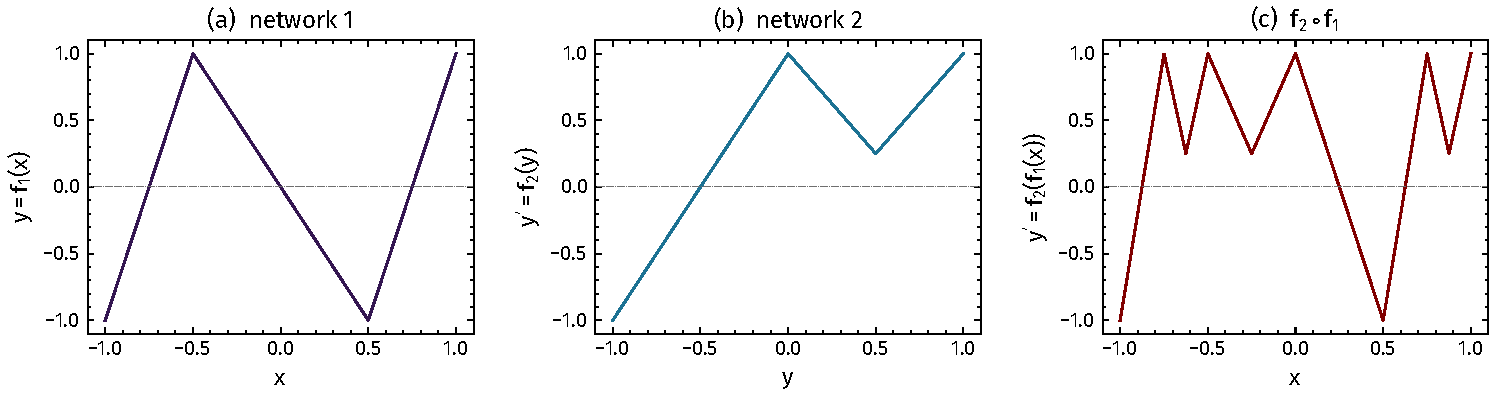
\includegraphics[height=0.445\textheight]{compose}
  \end{center}
  \figcap[0.95]{(a) $f_1$, a zigzag. (b) $f_2$, over the range that
  $f_1$ produces. (c) the composition $f_2\circ f_1$: $f_2$'s shape
  appears once per branch of $f_1$.}
  \vspace{0.1em}
  {\footnotesize
  \begin{itemize}\setlength{\itemsep}{1pt}
    \item Six hidden units in total, but the composition has far more
          joints than any six-unit shallow network could
  \end{itemize}}
\end{frame}

\begin{frame}{Why the pieces multiply}
  \begin{propx}[Composition of piecewise-linear maps]
    {\small If $f_1:\mathbb{R}\to\mathbb{R}$ is continuous and
    piecewise linear with $p$ pieces, and $f_2$ with $q$ pieces, then
    $f_2\circ f_1$ is continuous and piecewise linear with \alert{at
    most $pq$} pieces. The bound is attained when $f_1$ maps each of
    its pieces \emph{onto} the whole domain of $f_2$.}
  \end{propx}
  \vspace{0.1em}
  {\footnotesize
  \begin{itemize}\setlength{\itemsep}{2pt}
    \item \focus{1}{Let $I$ be one of the $p$ intervals on which
          $f_1$ is affine. On $I$, $f_2\circ f_1$ can change slope
          only where $f_1(x)$ crosses a breakpoint of $f_2$}
    \item \focus{2}{$f_1$ is affine on $I$, so it crosses each of the
          $q-1$ breakpoints of $f_2$ \alert{at most once} --- giving
          at most $q-1$ new breakpoints, hence at most $q$ pieces
          on $I$}
    \item \focus{3}{Summing over the $p$ intervals gives at most
          $pq$ pieces. Continuity is preserved because a composition
          of continuous maps is continuous \hfill $\square$}
    \item \focus{4}{Equality needs every piece of $f_1$ to sweep all
          of $f_2$'s breakpoints --- which is exactly what a
          \alert{fold} does}
  \end{itemize}}
\end{frame}

\begin{frame}{Folding: why the pattern repeats}
  \centering
  \begin{tikzpicture}[line width=0.9pt, scale=0.74]
    \draw[shc, fill=shc!8] (-3.4,1.5) rectangle (3.4,2.1);
    \foreach \x in {-1.13, 1.13}
      \draw[dpc, dashed] (\x,1.42) -- (\x,2.18);
    \node[font=\scriptsize, shc] at (-4.4,1.8) {input $x$};
    \node[font=\scriptsize, dpc] at (0,2.42) {fold lines};

    \draw[shc, line width=1.4pt]
      (-3.0,0.15) -- (-1.2,0.75) -- (0.6,0.15) -- (2.4,0.75);
    \node[font=\scriptsize, shc] at (-4.4,0.45) {folded};
    \node[font=\scriptsize, mcMuted, align=center]
      at (3.9,0.45) {three branches\\land on one range};

    \draw[tealc, fill=tealc!10] (-3.4,-1.0) rectangle (3.4,-0.4);
    \node[font=\scriptsize, tealc] at (-4.4,-0.7) {$f_2$ applied};
    \draw[tealc, line width=1.2pt]
      (-3.4,-0.95) .. controls (-1.5,-0.15) .. (0.0,-0.55)
                   .. controls (1.5,-0.95) .. (3.4,-0.45);

    \node[font=\scriptsize, dpc] at (-4.4,-2.1) {unfolded};
    \foreach \o in {-3.4,-1.13,1.13}{
      \draw[dpc, line width=1.0pt]
        (\o,-2.4) .. controls (\o+0.75,-1.7) .. (\o+1.13,-2.0)
                  .. controls (\o+1.7,-2.4) .. (\o+2.27,-1.9);
    }
    \draw[->, mcMuted] (0,1.35) -- (0,0.95);
    \draw[->, mcMuted] (0,-0.05) -- (0,-0.35);
    \draw[->, mcMuted] (0,-1.1) -- (0,-1.5);
  \end{tikzpicture}
  \vspace{0.4em}
  {\small
  \begin{itemize}\setlength{\itemsep}{2pt}
    \item $f_1$ \alert{folds} the input line: three different $x$
          land on the same $u$
    \item $f_2$ cannot tell them apart --- so its shape is stamped
          \alert{once per branch}
  \end{itemize}}
\end{frame}

\begin{frame}{The same thing, in the plots}
  \begin{center}
    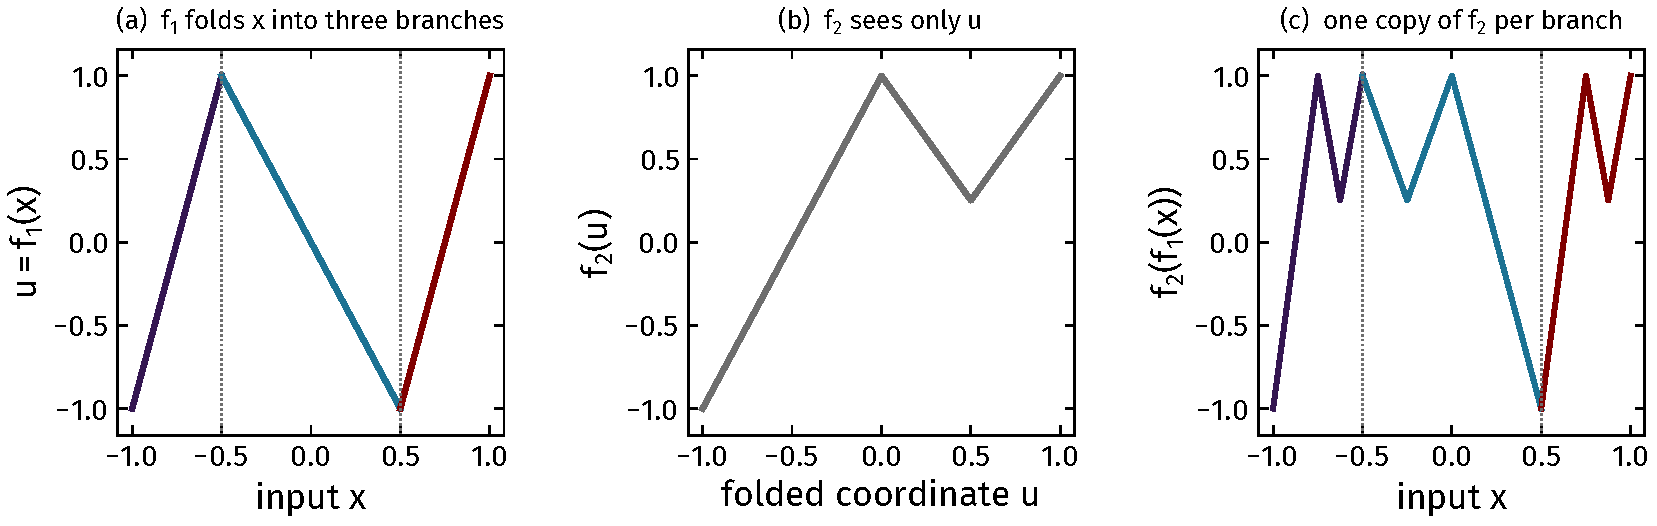
\includegraphics[height=0.475\textheight]{fold}
  \end{center}
  \figcap[0.95]{(a) the three branches of $f_1$, coloured. (b) $f_2$
  on the folded coordinate $u$. (c) the composition --- each branch
  carries its own copy of $f_2$, in the matching colour.}
  \shpar{joints \emph{add}: $M$ units $\to$ $M{+}1$ pieces}
        {folding \emph{multiplies} pieces across layers}
\end{frame}

\begin{frame}{Counting for our two networks}
  \vspace{0.3em}
  \begin{itemize}\setlength{\itemsep}{4pt}
    \item $f_1$ has $3$ hidden units, so $4$ pieces and
          \alert{$3$ monotone branches} on $[-1,1]$
    \item $f_2$ has $3$ hidden units, so \alert{$4$ pieces} on its
          input range
    \item By the Proposition the composition has up to
          $3\times 4 = \alert{12}$ pieces --- from only $6$ units
  \end{itemize}
  \vfill
  In general, for $L$ layers of $M$ units on a scalar input:
  \[
    \underbrace{ML + 1}_{\text{shallow, } ML \text{ units}}
    \qquad\text{versus}\qquad
    \underbrace{(M+1)^{L}}_{\text{deep, same unit count}}
  \]
  \vfill
  \begin{redhighlight}
    Width \alert{adds} pieces. Depth \alert{multiplies} them.
  \end{redhighlight}
\end{frame}

\begin{frame}{Composing in two dimensions}
  \begin{center}
    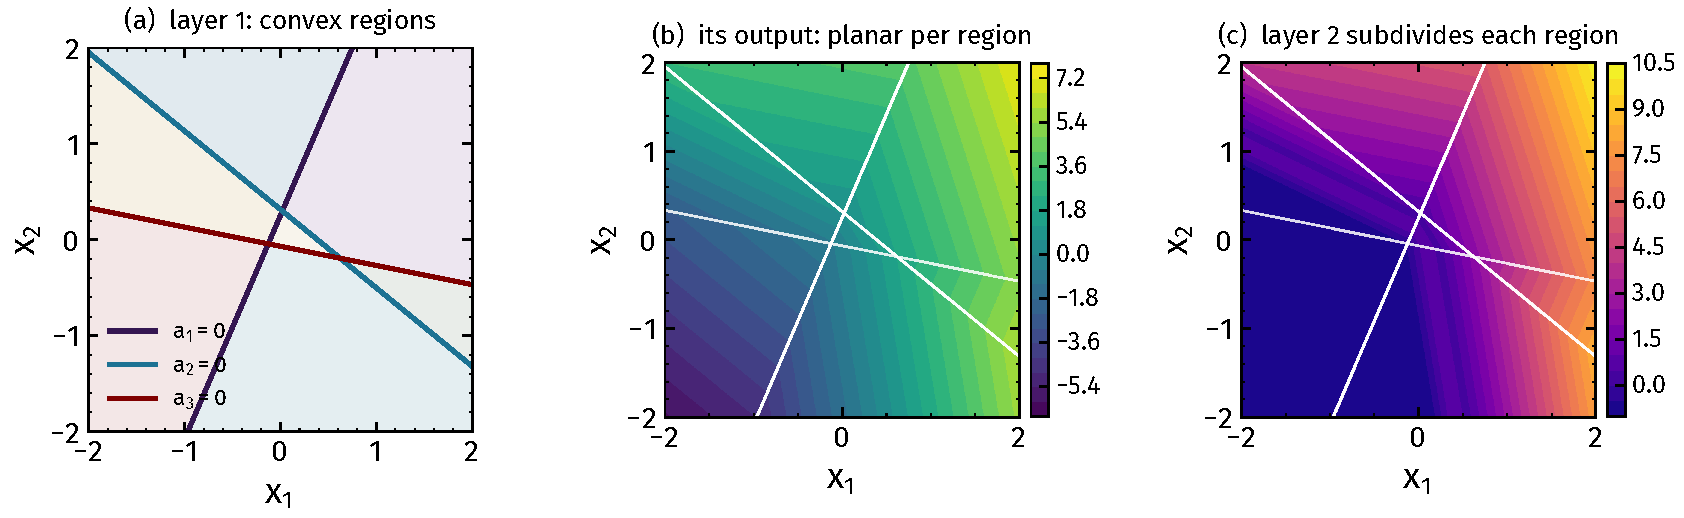
\includegraphics[height=0.435\textheight]{compose2d}
  \end{center}
  \figcap[0.96]{Layer 1 takes $\mathbf{x}=(x_1,x_2)$ into three ReLU
  units. (a) each unit contributes a line $a_j=0$; together they cut
  the plane into \emph{convex} regions, one per activation pattern.
  (b) the layer output is planar on each region. (c) layer 2 bends
  the values \emph{within} every region, subdividing each one.}
  \vspace{0.1em}
  {\footnotesize
  \begin{itemize}\setlength{\itemsep}{0pt}
    \item In 2-D the fold becomes a \alert{crease pattern}: depth
          creases an already-creased plane
  \end{itemize}}
\end{frame}

% =====================================================================
\section{The Deep Network}
% =====================================================================

\begin{frame}{Two hidden layers}
  \begin{columns}[T, onlytextwidth]
    \begin{column}{0.52\textwidth}
      \centering
      \begin{tikzpicture}[>=Stealth, line width=0.7pt,
          font=\small, scale=0.66, transform shape]
        \plainunit{x}{(0,0)}{black!55}{$x$}
        \unit{a1}{(2.0,1.45)}{shc}{}
        \unit{a2}{(2.0,0.0)}{shc}{}
        \unit{a3}{(2.0,-1.45)}{shc}{}
        \unit{b1}{(4.1,1.45)}{dpc}{}
        \unit{b2}{(4.1,0.0)}{dpc}{}
        \unit{b3}{(4.1,-1.45)}{dpc}{}
        \plainunit{y}{(6.1,0)}{black!55}{$\hat y$}
        \foreach \i in {1,2,3} \draw[->, black!45] (x)--(a\i);
        \foreach \i in {1,2,3} \foreach \j in {1,2,3}
          \draw[->, black!22] (a\i)--(b\j);
        \foreach \i in {1,2,3} \draw[->, black!45] (b\i)--(y);
        \node[font=\small, shc] at (2.0,2.55) {$\mathbf{z}^{(1)}$};
        \node[font=\small, dpc] at (4.1,2.55) {$\mathbf{z}^{(2)}$};
      \end{tikzpicture}
      \\[0.3em]
      \figsource{Each circle carries the activation $h$; arrows are
      weights.}
    \end{column}
    \hfill
    \begin{column}{0.44\textwidth}
      \vspace{0.4em}
      {\small Layer 1, layer 2, then the read-out:}
      \begin{align*}
        \mathbf{z}^{(1)} &= h\big(\mathbf{W}^{(1)}\mathbf{x}
                            + \mathbf{b}^{(1)}\big)\\
        \mathbf{z}^{(2)} &= h\big(\mathbf{W}^{(2)}\mathbf{z}^{(1)}
                            + \mathbf{b}^{(2)}\big)\\
        \hat y &= \mathbf{W}^{(3)}\mathbf{z}^{(2)} + \mathbf{b}^{(3)}
      \end{align*}
      {\small Each layer: a \alert{linear map} then an
      \alert{activation}. Our $f_2\circ f_1$ is exactly this, with
      $h=\mathrm{ReLU}$.}
    \end{column}
  \end{columns}
  \shpar{one hidden layer}
        {hidden layers \emph{stacked}: the same block, composed}
\end{frame}

\begin{frame}{Computed step by step}
  \begin{center}
    
\includegraphics[height=0.565\textheight]{buildup}
  \end{center}
  \vspace{-0.1em}
  \figcap[0.97]{(a--c) each unit of layer 1: dashed $a^{(1)}_j$,
  solid $z^{(1)}_j$. (d) scaled by the second-layer weights.
  (e) summed: $f_1$. (f) pushed through layer 2.}
\end{frame}

\begin{frame}{The general deep network}
  \centering
  \begin{tikzpicture}[>=Stealth, line width=0.6pt, font=\small,
      scale=0.60, transform shape]
    \plainunit{x1}{(0,0.75)}{black!55}{}
    \plainunit{x2}{(0,-0.75)}{black!55}{}
    \node[font=\small] at (0,1.85) {$\mathbf{x}$};
    \node[font=\scriptsize, mcMuted] at (0,-1.7) {$D=2$};
    \foreach \L/\c/\xx in {1/shc/2.3, 2/tealc/4.6, 3/dpc/6.9}{
      \foreach \i/\yy in {1/1.55, 2/0.0, 3/-1.55}
        \unit{l\L-\i}{(\xx,\yy)}{\c}{};
      \node[font=\small] at (\xx,2.45) {$\mathbf{z}^{(\L)}$};
      \node[font=\scriptsize, mcMuted] at (\xx,-2.42) {$M=3$};
    }
    \plainunit{y1}{(9.2,0.75)}{black!55}{}
    \plainunit{y2}{(9.2,-0.75)}{black!55}{}
    \node[font=\small] at (9.2,1.85) {$\hat{\mathbf{y}}$};
    \node[font=\scriptsize, mcMuted] at (9.2,-1.7) {$K=2$};
    \foreach \i in {1,2} \foreach \j in {1,2,3}
      \draw[->, black!22] (x\i)--(l1-\j);
    \foreach \i in {1,2,3} \foreach \j in {1,2,3}{
      \draw[->, black!18] (l1-\i)--(l2-\j);
      \draw[->, black!18] (l2-\i)--(l3-\j);
    }
    \foreach \i in {1,2,3} \foreach \j in {1,2}
      \draw[->, black!22] (l3-\i)--(y\j);
    \node[font=\scriptsize, shc]   at (1.15,-3.05)
      {$\mathbf{W}^{(1)},\mathbf{b}^{(1)}$};
    \node[font=\scriptsize, tealc] at (3.45,-3.05)
      {$\mathbf{W}^{(2)},\mathbf{b}^{(2)}$};
    \node[font=\scriptsize, dpc]   at (5.75,-3.05)
      {$\mathbf{W}^{(3)},\mathbf{b}^{(3)}$};
    \node[font=\scriptsize, black!60] at (8.05,-3.05)
      {$\mathbf{W}^{(4)},\mathbf{b}^{(4)}$};
  \end{tikzpicture}
  \vspace{0.2em}
  \begin{columns}[T, onlytextwidth]
    \begin{column}{0.44\textwidth}
      \vspace{-0.4em}
      \[
        \mathbf{z}^{(l)} = h\big(\mathbf{W}^{(l)}\mathbf{z}^{(l-1)}
        + \mathbf{b}^{(l)}\big)
      \]
    \end{column}
    \hfill
    \begin{column}{0.52\textwidth}
      {\footnotesize
      \begin{itemize}\setlength{\itemsep}{0pt}
        \item $\mathbf{z}^{(0)}=\mathbf{x}$, and $h$ acts
              element-wise
        \item \alert{Depth} $L$ $=$ hidden layers ($3$ here);
              \alert{width} $M$ $=$ units per layer --- both
              \alert{hyperparameters}
        \item Parameters here: $9+12+12+8=41$
      \end{itemize}}
    \end{column}
  \end{columns}
\end{frame}

\begin{frame}{Building depth recursively}
  \vspace{0.2em}
  The two-layer construction \alert{extends recursively}
  (Bishop \& Bishop, 2024, \S6.2):
  \[
    \mathbf{z}^{(1)} = h\big(\mathbf{W}^{(1)}\mathbf{x}\big),
    \quad
    \mathbf{z}^{(2)} = h\big(\mathbf{W}^{(2)}\mathbf{z}^{(1)}\big),
    \quad \dots, \quad
    \hat{\mathbf{y}} = \mathbf{W}^{(L+1)}\mathbf{z}^{(L)}
  \]
  \vspace{-0.2em}
  {\small (biases absorbed by a clamped unit $z^{(l)}_0=1$)}
  \vfill
  {\small
  \begin{itemize}\setlength{\itemsep}{3pt}
    \item Each layer feeds the next --- the \alert{same operation}
          (linear map, then nonlinearity) repeated
    \item Nothing new is needed: depth is \alert{repetition of a
          single idea}
  \end{itemize}}
  \shpar{$\hat y = \mathbf{W}^{(2)}h(\mathbf{W}^{(1)}\mathbf{x})$}
        {$\hat y = \mathbf{W}^{(L+1)}h(\cdots
         h(\mathbf{W}^{(1)}\mathbf{x}))$}
\end{frame}

\begin{frame}{A note on counting layers}
  \centering
  \begin{tikzpicture}[>=Stealth, line width=0.6pt, font=\small,
      scale=0.66, transform shape]
    \plainunit{i1}{(0,0.75)}{black!55}{}
    \plainunit{i2}{(0,-0.75)}{black!55}{}
    \unit{m1}{(2.5,0.75)}{shc}{}
    \unit{m2}{(2.5,-0.75)}{shc}{}
    \plainunit{o1}{(5.0,0)}{black!55}{}
    \foreach \i in {1,2} \foreach \j in {1,2}
      \draw[->, black!25] (i\i)--(m\j);
    \foreach \i in {1,2} \draw[->, black!25] (m\i)--(o1);
    \node[font=\scriptsize] at (0,-1.6) {inputs};
    \node[font=\scriptsize, shc] at (2.5,-1.6) {hidden};
    \node[font=\scriptsize] at (5.0,-1.6) {output};
    \draw[decorate, decoration={brace, amplitude=4pt},
          mcMuted] (-0.5,1.6) -- (5.5,1.6)
      node[midway, above=4pt, font=\scriptsize, mcMuted]
      {3 layers \emph{of units}};
    \draw[decorate, decoration={brace, amplitude=4pt, mirror},
          dpc] (0.6,-2.15) -- (4.4,-2.15)
      node[midway, below=4pt, font=\scriptsize, dpc]
      {2 layers \emph{of weights}};
  \end{tikzpicture}
  \vspace{0.3em}
  {\small
  \begin{itemize}\setlength{\itemsep}{2pt}
    \item The same network is called ``three-layer'',
          ``single-hidden-layer'' or ``two-layer'' depending on what
          is counted
    \item Bishop counts \alert{layers of weights} --- the adaptive
          parameters \hfill{\scriptsize B\&B (2024), \S6.3}
    \item In this course: \alert{deep} means more than one hidden
          layer, i.e.\ $L>1$
  \end{itemize}}
\end{frame}

% =====================================================================
\section{Universal Approximation}
% =====================================================================

\begin{frame}{What we already proved, and what is missing}
  \begin{lemmax}[One dimension, from Class 5]
    {\small For every continuous $f$ on $[a,b]$ and every
    $\varepsilon>0$ there is a \alert{one-hidden-layer} ReLU network
    $\hat y$ with finitely many units such that
    $\sup_{x\in[a,b]}|f(x)-\hat y(x)|<\varepsilon$.}
  \end{lemmax}
  \vspace{0.2em}
  {\small
  \begin{itemize}\setlength{\itemsep}{3pt}
    \item We proved this \alert{constructively}: two ReLUs make a
          ramp, slope increments reproduce the piecewise-linear
          interpolant exactly, uniform continuity bounds the error
    \item What is missing is the general case: $D$ inputs, and an
          arbitrary non-polynomial activation
  \end{itemize}}
  \vspace{0.3em}
  \begin{redhighlight}
    {\small The route to $D$ dimensions is to reduce it to the
    one-dimensional case, using functions that vary along a
    \alert{single direction}.}
  \end{redhighlight}
\end{frame}

\begin{frame}{Ridge functions}
  \vspace{0.2em}
  A \alert{ridge function} is one that depends on $\mathbf{x}$ only
  through a single linear combination:
  \[
    \mathbf{x} \;\longmapsto\; g\big(\mathbf{w}^{\!\top}\mathbf{x}+b\big),
    \qquad \mathbf{w}\in\mathbb{R}^{D},\; b\in\mathbb{R}
  \]
  \vfill
  {\small
  \begin{itemize}\setlength{\itemsep}{4pt}
    \item It is \alert{constant} on every hyperplane perpendicular to
          $\mathbf{w}$ --- all of its variation is along one
          direction
    \item \alert{Every hidden unit of a network is a ridge
          function}: $h(\mathbf{w}_j^{\!\top}\mathbf{x}+w_{j0})$
    \item So a one-hidden-layer network is exactly a \alert{finite
          sum of ridge functions}
  \end{itemize}}
  \vspace{0.1em}
  \begin{redhighlight}
    {\footnotesize If sums of ridge functions reach any continuous
    function, and Lemma 1 reproduces any \emph{one-dimensional}
    profile, we are done.}
  \end{redhighlight}
\end{frame}

\begin{frame}{Ridge functions are enough}
  \begin{lemmax}[Density of trigonometric ridge functions]
    {\small Let $\mathcal{K}\subset\mathbb{R}^{D}$ be compact. The set
    \[
      \mathcal{R} = \Big\{\, \mathbf{x}\mapsto
      \textstyle\sum_{k=1}^{K} c_k
      \cos\big(\mathbf{w}_k^{\!\top}\mathbf{x}+b_k\big)
      \;:\; K\in\mathbb{N},\; c_k,b_k\in\mathbb{R},\;
      \mathbf{w}_k\in\mathbb{R}^{D} \Big\}
    \]
    is dense in $C(\mathcal{K})$ under the supremum norm.}
  \end{lemmax}
  \vspace{-0.2em}
  {\scriptsize
  \emph{Proof} (Stone--Weierstrass; check the three hypotheses).
  \begin{itemize}\setlength{\itemsep}{1pt}
    \item \focus{1}{\textbf{Algebra.} $\mathcal{R}$ is closed under
          products, because
          $\cos A\cos B=\tfrac12\big[\cos(A-B)+\cos(A+B)\big]$ turns
          a product of two ridge terms into a sum of two more}
    \item \focus{2}{\textbf{Constants.} Take
          $\mathbf{w}=\mathbf{0}$, $b=0$: the constant function $1$
          lies in $\mathcal{R}$}
    \item \focus{3}{\textbf{Separates points.} For
          $\mathbf{x}\ne\mathbf{y}$ choose $\mathbf{w}$ with
          $t=\mathbf{w}^{\!\top}(\mathbf{x}-\mathbf{y})\in(0,\pi)$;
          then $\cos(\mathbf{w}^{\!\top}\mathbf{x})\ne
          \cos(\mathbf{w}^{\!\top}\mathbf{y})$ for a suitable
          offset}
    \item \focus{4}{Stone--Weierstrass then gives density in
          $C(\mathcal{K})$ \hfill $\square$}
  \end{itemize}}
\end{frame}

\begin{frame}{Universal approximation in $D$ dimensions}
  \begin{theorem}[Cybenko 1989; Hornik 1991]
    {\small Let $h$ be continuous and \alert{not a polynomial},
    $\mathcal{K}\subset\mathbb{R}^{D}$ compact and
    $f\in C(\mathcal{K})$. For every $\varepsilon>0$ there exist
    $M\in\mathbb{N}$ and weights such that
    \[
      \hat y(\mathbf{x}) = w^{(2)}_0 + \sum_{j=1}^{M} w^{(2)}_j\,
      h\big(\mathbf{w}_j^{(1)\top}\mathbf{x}+w^{(1)}_{j0}\big)
      \quad\text{satisfies}\quad
      \sup_{\mathbf{x}\in\mathcal{K}}\big|f(\mathbf{x})
      -\hat y(\mathbf{x})\big|<\varepsilon .
    \]}
  \end{theorem}
  \vspace{0.1em}
  {\footnotesize
  \begin{itemize}\setlength{\itemsep}{1pt}
    \item \focus{1}{\textbf{Step 1.} By Lemma 2 pick
          $g=\sum_{k=1}^{K}c_k\cos(\mathbf{w}_k^{\!\top}\mathbf{x}
          +b_k)$ with $\sup_{\mathcal{K}}|f-g|<\varepsilon/2$}
    \item \focus{2}{\textbf{Step 2.} As $\mathbf{x}$ ranges over the
          compact $\mathcal{K}$, each
          $t_k=\mathbf{w}_k^{\!\top}\mathbf{x}+b_k$ ranges over a
          \alert{compact interval} $I_k$}
    \item \focus{3}{\textbf{Step 3.} By Lemma 1 approximate
          $\cos$ on $I_k$ by
          $\sum_j \alpha_{kj}h(\beta_{kj}t+\gamma_{kj})$ to within
          $\varepsilon/(2K|c_k|)$}
    \item \focus{4}{\textbf{Step 4.} Substitute
          $t=\mathbf{w}_k^{\!\top}\mathbf{x}+b_k$. Then
          $h(\beta_{kj}t+\gamma_{kj})
          =h(\tilde{\mathbf{w}}^{\!\top}\mathbf{x}+\tilde w_0)$ ---
          still \alert{one hidden layer}. Summing over $k$ and
          applying the triangle inequality gives
          $\varepsilon/2+\varepsilon/2$ \hfill $\square$}
  \end{itemize}}
\end{frame}

\begin{frame}{The construction, drawn}
  \begin{columns}[T, onlytextwidth]
    \begin{column}{0.52\textwidth}
      \centering
      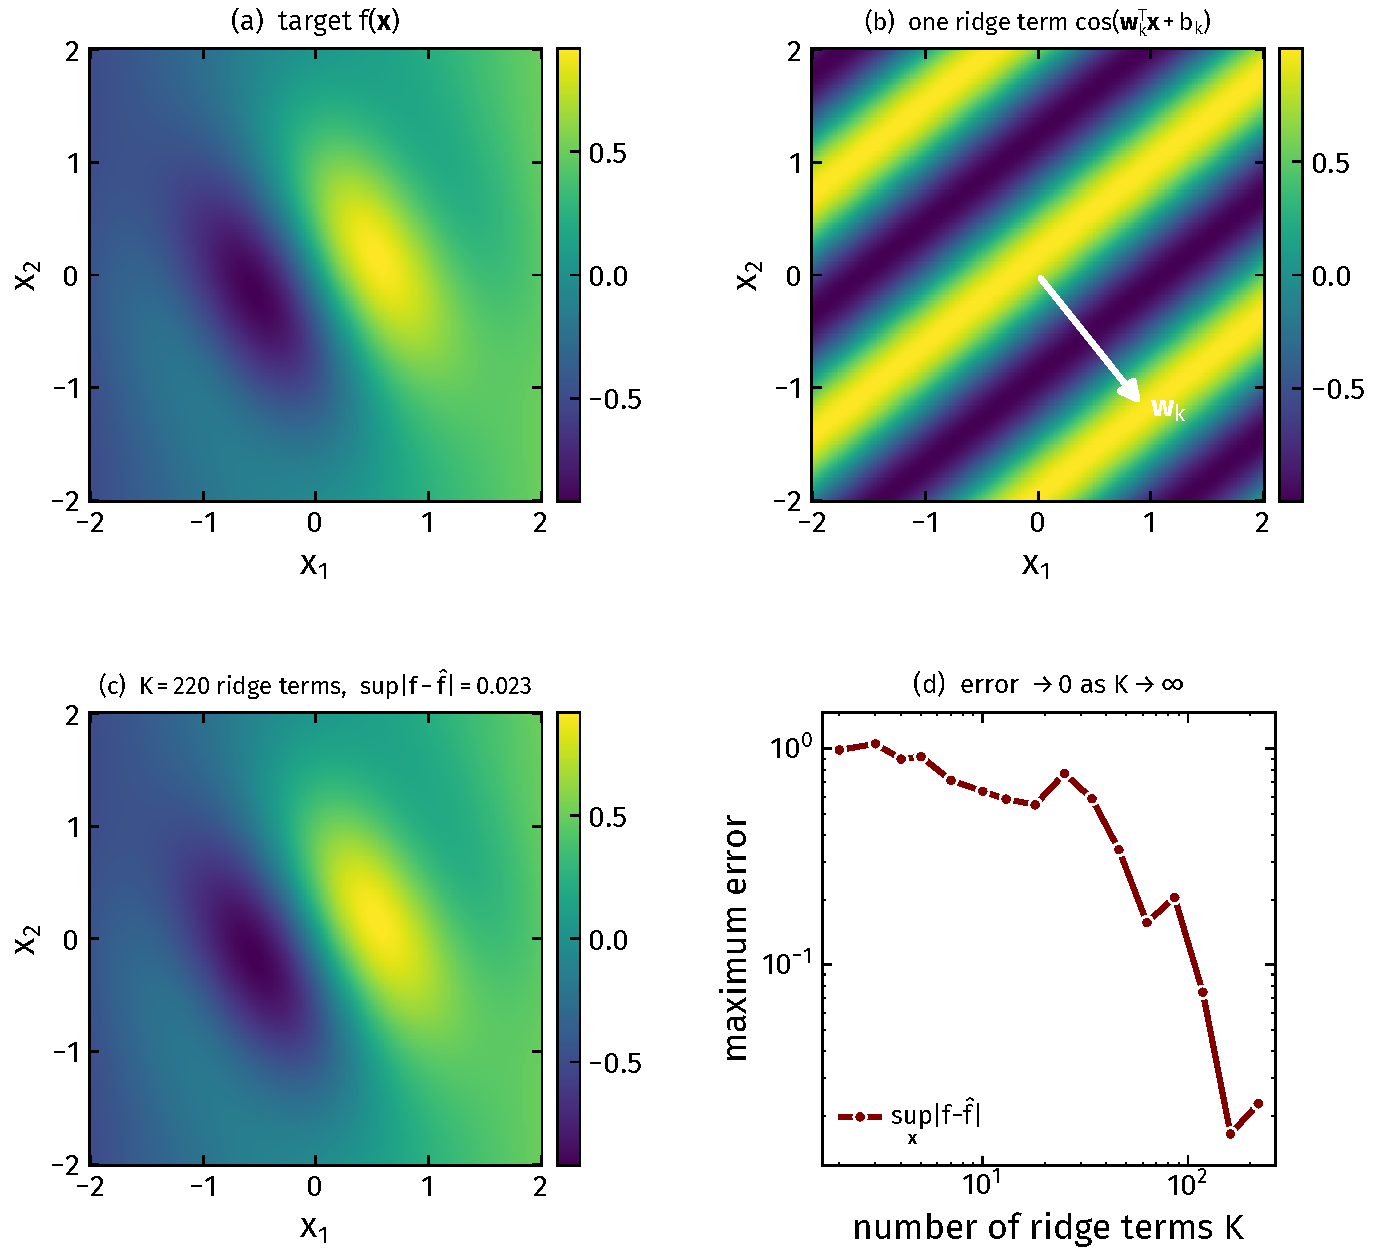
\includegraphics[height=0.72\textheight]{ua_ridge}
    \end{column}
    \hfill
    \begin{column}{0.44\textwidth}
      \vspace{0.4em}
      {\small
      \begin{itemize}\setlength{\itemsep}{5pt}
        \item (a) a continuous target on a compact square
        \item (b) \emph{one} ridge term: constant along the
              directions perpendicular to $\mathbf{w}_k$
        \item (c) $K=220$ such terms, fitted by least squares ---
              already indistinguishable from the target
        \item (d) the error falls steadily as $K$ grows, which is
              Step 1 of the proof in action
      \end{itemize}}
    \end{column}
  \end{columns}
\end{frame}

\begin{frame}{Which activations work?}
  \begin{theorem}[Leshno, Lin, Pinkus \& Schocken, 1993]
    {\small For continuous $h$, one-hidden-layer networks are dense in
    $C(\mathcal{K})$ for every compact $\mathcal{K}$ \alert{if and
    only if} $h$ is \alert{not a polynomial}.}
  \end{theorem}
  \vspace{0.1em}
  {\footnotesize
  \emph{Proof of the ``only if'' direction.} Suppose $h$ is a
  polynomial of degree $p$. Then
  $h(\mathbf{w}^{\!\top}\mathbf{x}+w_0)$ is a polynomial in
  $\mathbf{x}$ of degree at most $p$, and any finite sum of such
  terms is too. So every network output lies in the
  \alert{finite-dimensional} space of polynomials of degree
  $\le p$, which is closed and is not all of $C(\mathcal{K})$.
  No amount of width escapes it. \hfill$\square$}
  \vspace{0.3em}
  {\small
  \begin{itemize}\setlength{\itemsep}{3pt}
    \item This is exactly the Class 5 observation that without a
          nonlinearity the network \alert{collapses to a line}, in
          its sharpest form
    \item ReLU, $\tanh$, sigmoid, softplus and GELU all qualify;
          $h(a)=a^2$ does not
  \end{itemize}}
\end{frame}

\begin{frame}{What ReLU networks compute, exactly}
  \begin{propx}[ReLU networks are the piecewise-linear functions]
    {\small (i) Every ReLU network computes a \alert{continuous
    piecewise-linear} function. (ii) Conversely, every continuous
    piecewise-linear $f:\mathbb{R}^{D}\to\mathbb{R}$ is computed
    \alert{exactly} by a ReLU network with at most
    $\lceil\log_2(D{+}1)\rceil$ hidden layers.
    \hfill{\scriptsize (ii): Arora et al., 2018}}
  \end{propx}
  \vspace{0.1em}
  {\footnotesize
  \emph{Proof of (i), by induction on the layer index.} The identity
  map is piecewise linear. If $\mathbf{z}^{(l-1)}$ is piecewise
  linear then so is $\mathbf{W}^{(l)}\mathbf{z}^{(l-1)}
  +\mathbf{b}^{(l)}$, since affine maps and sums of piecewise-linear
  functions are piecewise linear; and $h=\max(0,\cdot)$ is itself
  piecewise linear, so the composition is too. Continuity is
  preserved at every step. \hfill$\square$}
  \vspace{-0.1em}
  \begin{redhighlight}
    {\scriptsize Depth does \alert{not} enlarge the class a ReLU
    network can represent --- shallow and deep both give exactly the
    continuous piecewise-linear functions. What changes is
    \alert{how many units} it costs.}
  \end{redhighlight}
\end{frame}

\begin{frame}{What universality does \emph{not} settle}
  \vspace{0.2em}
  \begin{itemize}\setlength{\itemsep}{5pt}
    \item \alert{It is an existence result.} Good weights exist; it
          says nothing about whether gradient descent finds them
    \item \alert{It says nothing about generalisation.} Fitting a
          training set is not the goal
    \item \alert{It gives no useful size bound.} The grid argument
          in $D$ dimensions needs
          $M=O\big((L_{\!f}/\varepsilon)^{D}\big)$ units
    \item \alert{Both shallow and deep networks are universal}, so
          universality cannot be the reason to prefer depth
  \end{itemize}
  \vspace{0.4em}
  \begin{redhighlight}
    The right question is not \emph{whether} a network can represent
    a function, but \alert{how efficiently}.
  \end{redhighlight}
\end{frame}

% =====================================================================
\section{Depth versus Width}
% =====================================================================

\begin{frame}{A function that depth computes cheaply}
  \begin{lemmax}[The sawtooth]
    {\small Let $T(x)=2h(x)-4h(x-\tfrac12)$, a \alert{two-unit} ReLU
    network. Then $T$ maps $[0,1]$ onto $[0,1]$, folding it in half,
    and the $L$-fold composition $T^{\circ L}$ is piecewise linear
    with \alert{exactly $2^{L}$ pieces}, computed by a ReLU network
    of depth $L$ and width $2$.}
  \end{lemmax}
  \vspace{0.1em}
  {\footnotesize
  \begin{itemize}\setlength{\itemsep}{2pt}
    \item \focus{1}{$T(x)=2x$ on $[0,\tfrac12]$ and $T(x)=2-2x$ on
          $[\tfrac12,1]$: each half is mapped \alert{affinely onto
          all of} $[0,1]$}
    \item \focus{2}{\textbf{Base case.} $T^{\circ 1}=T$ has
          $2^{1}=2$ pieces}
    \item \focus{3}{\textbf{Induction.} Write
          $T^{\circ L}=T^{\circ(L-1)}\circ T$. On each half of
          $[0,1]$, $T$ is affine and onto, so $T^{\circ L}$
          restricted there is a rescaled copy of $T^{\circ(L-1)}$,
          contributing $2^{L-1}$ pieces}
    \item \focus{4}{Two halves give $2\cdot 2^{L-1}=2^{L}$ pieces
          \hfill $\square$}
  \end{itemize}}
\end{frame}

\begin{frame}{The sawtooth, drawn}
  \begin{columns}[T, onlytextwidth]
    \begin{column}{0.53\textwidth}
      \centering
      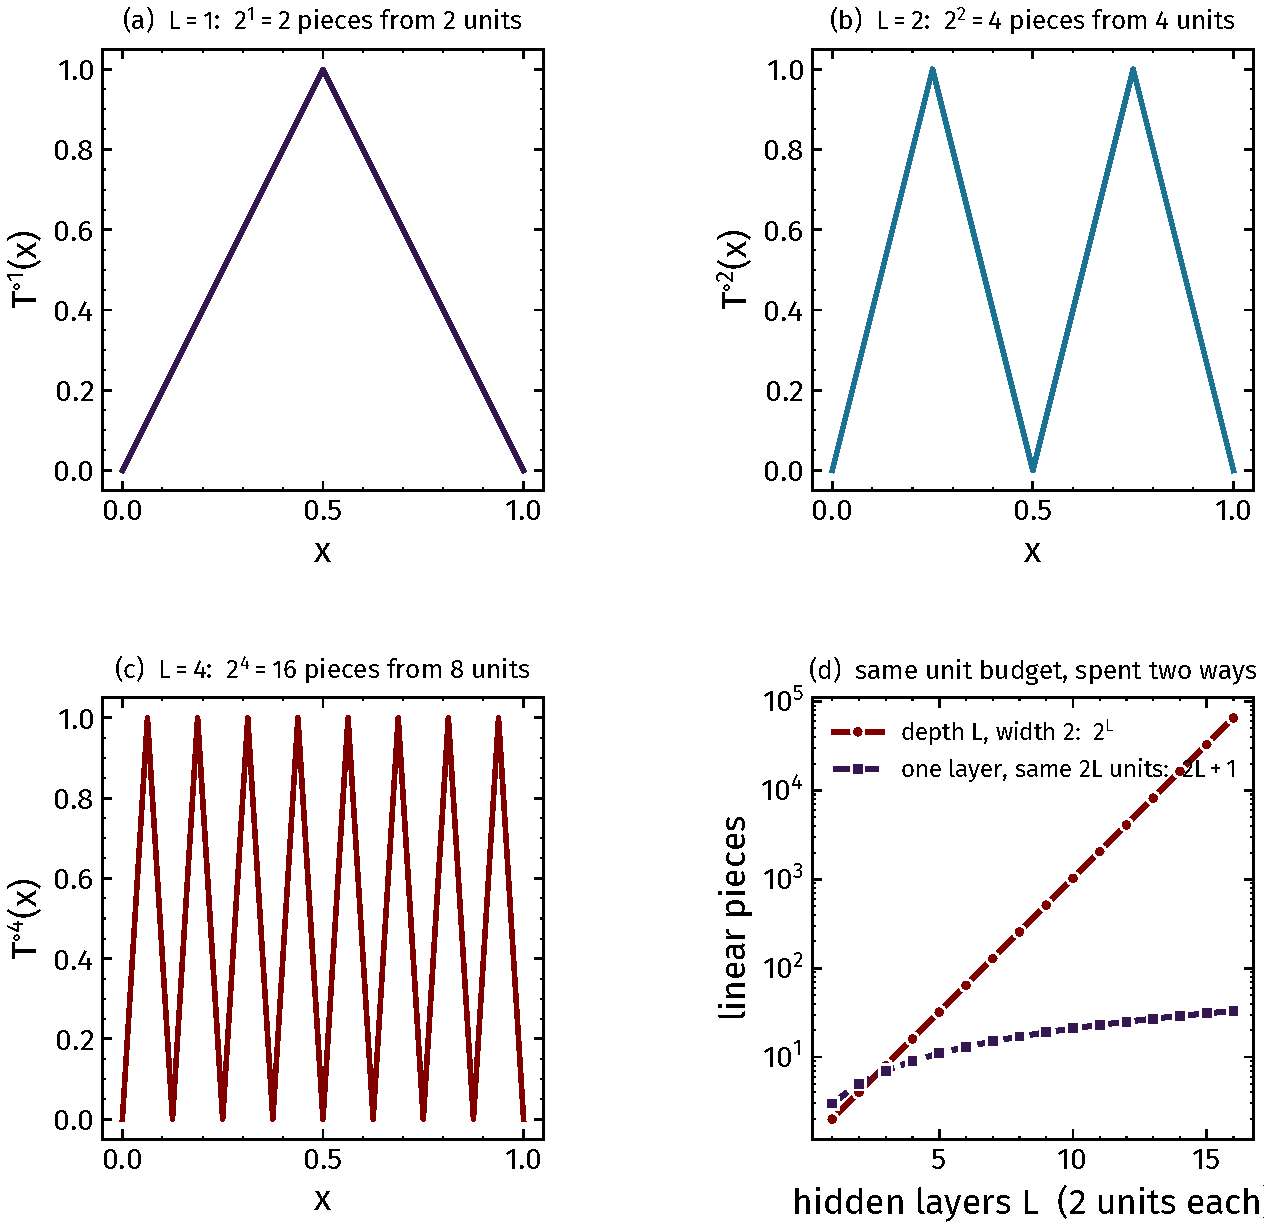
\includegraphics[height=0.72\textheight]{sawtooth}
    \end{column}
    \hfill
    \begin{column}{0.43\textwidth}
      \vspace{0.5em}
      {\small
      \begin{itemize}\setlength{\itemsep}{5pt}
        \item (a--c) each extra layer \alert{doubles} the number of
              teeth, at a cost of two more units
        \item (d) the same total budget of $2L$ units: spent as
              depth it buys $2^{L}$ pieces, spent as width only
              $2L+1$
        \item By $L=16$ that is $65{,}536$ against $33$
      \end{itemize}}
    \end{column}
  \end{columns}
\end{frame}

\begin{frame}{Depth beats width, provably}
  \begin{theorem}[Depth--width separation; after Telgarsky, 2016]
    {\small For every $L\in\mathbb{N}$ the function $T^{\circ L}$ is
    computed by a ReLU network with $L$ hidden layers of width $2$,
    that is $O(L)$ parameters. Any \alert{one-hidden-layer} ReLU
    network computing $T^{\circ L}$ exactly needs at least
    $2^{L}-1$ units.}
  \end{theorem}
  \vspace{-0.2em}
  {\scriptsize
  \begin{itemize}\setlength{\itemsep}{1pt}
    \item \focus{1}{From Class 5: a one-hidden-layer ReLU network
          with $M$ units on a scalar input is piecewise linear with
          at most $M+1$ pieces}
    \item \focus{2}{By the Lemma, $T^{\circ L}$ has exactly $2^{L}$
          pieces}
    \item \focus{3}{Matching them requires $M+1\ge 2^{L}$, hence
          $M\ge 2^{L}-1$ \hfill $\square$}
    \item \focus{4}{Telgarsky's full theorem strengthens this from
          \emph{exact} representation to \emph{approximation}: no
          shallow network of sub-exponential size can even come
          close}
  \end{itemize}}
  \vspace{0.1em}
  \begin{redhighlight}
    {\footnotesize An \alert{exponential} gap, from a function you
    can draw in one line.}
  \end{redhighlight}
\end{frame}

\begin{frame}{The same effect in $D$ dimensions}
  \begin{theorem}[Region lower bound; Mont\'ufar et al., 2014]
    {\small A ReLU network with $L$ hidden layers of width
    $M\ge D$ on $\mathbb{R}^{D}$ can realise at least
    \[
      \Big(\prod_{l=1}^{L-1}\big\lfloor M/D \big\rfloor^{D}\Big)
      \sum_{j=0}^{D}\binom{M}{j}
    \]
    linear regions --- \alert{exponential in the depth $L$}, but only
    \alert{polynomial in the width $M$}.}
  \end{theorem}
  \vspace{0.1em}
  {\footnotesize
  \begin{itemize}\setlength{\itemsep}{2pt}
    \item The mechanism is the folding argument, iterated: each
          layer folds the already-folded input space
    \item The trailing $\sum_{j\le D}\binom{M}{j}$ is exactly the
          \alert{Zaslavsky count} from Class 5 --- the last layer
          behaves like a shallow network
    \item Lower bound only: it says such networks \emph{exist}, not
          that training finds them
  \end{itemize}}
\end{frame}

\begin{frame}{Linear regions per parameter}
  \begin{center}
    
\includegraphics[height=0.435\textheight]{regions}
  \end{center}
  \figcap[0.96]{Counts for a $1$-input, $1$-output ReLU network:
  $P_{\text{shallow}}(M)=3M+1$ and
  $P_{\text{deep}}(M,L)=2M+(L{-}1)M(M{+}1)+M+1$, with $M{+}1$ and
  $(M{+}1)^{L}$ regions. (a) regions bought per parameter, log--log.
  (b) a \emph{fixed} budget $P$: for each $L$ we take the widest $M$
  that still fits, then plot the regions it buys.}
  \shpar{regions grow \emph{polynomially} with width}
        {regions grow \emph{exponentially} with depth}
\end{frame}

\begin{frame}{Shallow vs.\ deep: the trade-off}
  \centering
  \vspace{0.3em}
  \renewcommand{\arraystretch}{1.2}
  {\footnotesize
  \begin{tabular}{p{0.24\textwidth} p{0.32\textwidth}
                  p{0.34\textwidth}}
    & \textbf{\color{shc}Shallow ($L=1$)}
    & \textbf{\color{dpc}Deep ($L>1$)}\\
    \hline
    Function class & continuous piecewise linear
      & \alert{the same} class\\
    Expressivity & universal, but may need $2^{L}$ units
      & universal with \alert{$O(L)$} units\\
    Regions & polynomial in width
      & exponential in depth\\
    Features & one level of learned features
      & \alert{hierarchical} features, layer on layer\\
    Training & convex read-out only
      & harder landscape; needs backpropagation\\
    \hline
  \end{tabular}}
  \vspace{0.5em}
  \begin{redhighlight}
    {\footnotesize Depth trades a harder optimisation problem for a
    dramatic gain in representational efficiency.}
  \end{redhighlight}
\end{frame}

% =====================================================================
\section{What Deep Networks Represent}
% =====================================================================

\begin{frame}{Depth as an inductive bias}
  \vspace{0.2em}
  \begin{itemize}\setlength{\itemsep}{5pt}
    \item Universality tells us what a network \emph{can} represent;
          it says nothing about what it \emph{prefers} to learn
    \item A deep architecture encodes an \alert{inductive bias}: that
          the output relates to the input through a \alert{hierarchy}
          of intermediate concepts \hfill{\scriptsize B\&B, \S6.3.1}
    \item For images, the map from pixels to a concept like `cat' is
          \alert{highly nonlinear} --- hopeless for one layer,
          natural for many
    \item The right bias means the network needs \alert{less data}
          and generalises better
  \end{itemize}
  \shpar{bias: the output is one nonlinear map of the input}
        {bias: the output is a \alert{hierarchy} of simpler maps}
\end{frame}

\begin{frame}{Hierarchical representations}
  \centering
  \vspace{0.5em}
  \begin{tikzpicture}[>=Stealth, line width=0.8pt,
      b/.style={rounded corners=3pt, draw=dpc, fill=dpc!7,
                align=center, minimum height=0.9cm,
                inner xsep=5pt, font=\small},
      lbl/.style={font=\scriptsize\itshape, mcMuted}]
    \node[b] (a) {pixels};
    \node[b, right=9mm of a] (b) {edges};
    \node[b, right=9mm of b] (c) {motifs\\ / parts};
    \node[b, right=9mm of c] (d) {objects};
    \node[b, right=9mm of d] (e) {`cat'};
    \draw[->] (a)--(b); \draw[->] (b)--(c);
    \draw[->] (c)--(d); \draw[->] (d)--(e);
    \node[lbl, below=1mm of a] {input};
    \node[lbl, below=1mm of b] {layer 1};
    \node[lbl, below=1mm of c] {layer 2};
    \node[lbl, below=1mm of d] {layer 3};
    \node[lbl, below=1mm of e] {output};
  \end{tikzpicture}
  \vspace{0.8em}
  {\small
  \begin{itemize}\setlength{\itemsep}{3pt}
    \item Early layers detect \alert{low-level} features; later
          layers assemble them into \alert{high-level} concepts
    \item Each layer reuses the layer below --- features are
          \alert{shared} by everything built on top
          \hfill{\scriptsize B\&B, \S6.3.1}
  \end{itemize}}
\end{frame}

\begin{frame}{Why hierarchy is the right bias for real data}
  \begin{columns}[T, onlytextwidth]
    \begin{column}{0.44\textwidth}
      \centering
      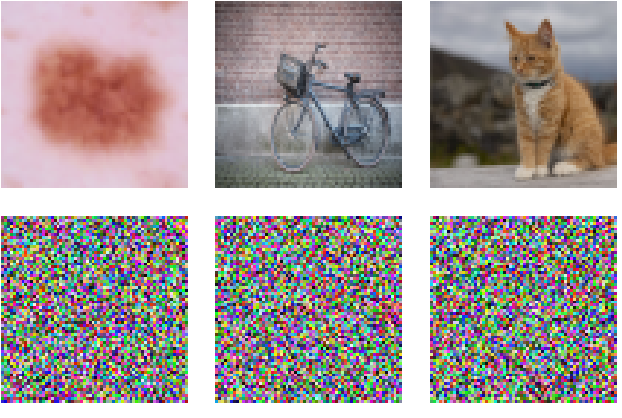
\includegraphics[height=0.44\textheight]{Bishop6_8}
      \\[0.1em]
      \figsource{Figure from Bishop \& Bishop (2024), Fig.~6.8:
      natural images (top) vs.\ random pixels (bottom).}
    \end{column}
    \hfill
    \begin{column}{0.52\textwidth}
      \vspace{0.4em}
      {\small
      \begin{itemize}\setlength{\itemsep}{4pt}
        \item Almost every random pixel pattern is \alert{noise} ---
              images like the one above are vanishingly rare among
              all possible images
        \item Natural data lives on a \alert{low-dimensional
              manifold} with strong structure
        \item That structure is \alert{compositional}, so a
              compositional model captures it efficiently
      \end{itemize}}
    \end{column}
  \end{columns}
\end{frame}

\begin{frame}{A hierarchy, built explicitly}
  \begin{center}
    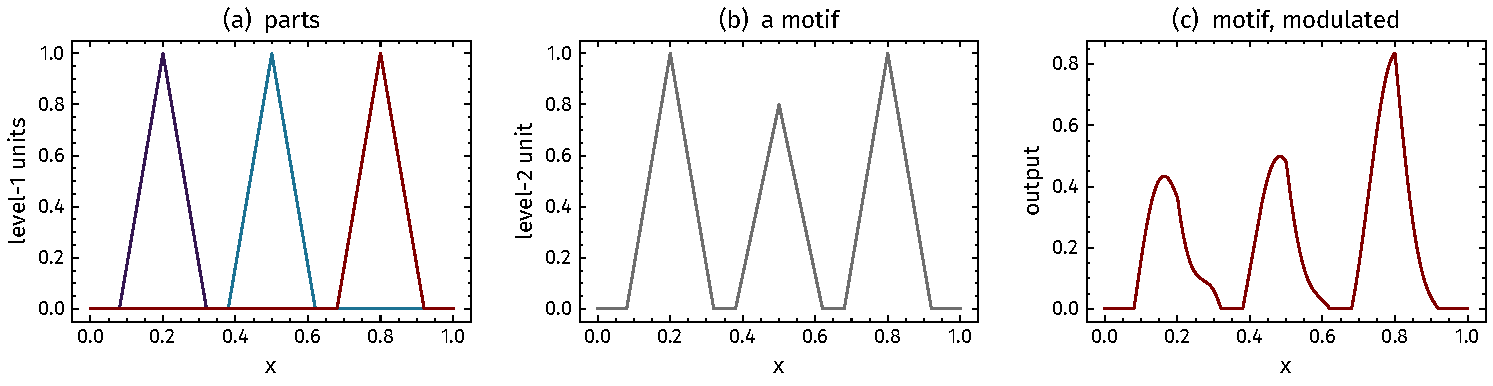
\includegraphics[height=0.485\textheight]{hierarchy}
  \end{center}
  \figcap[0.96]{(a) three level-1 units, each a bump
  $h(1-|x-c|/w)$ centred at $c\in\{0.2,0.5,0.8\}$ with $w=0.12$.
  (b) a level-2 unit sums them into one motif. (c) level 3 modulates
  that motif by $0.6+0.4\sin(6\pi x)$.}
  \vspace{0.1em}
  {\footnotesize
  \begin{itemize}\setlength{\itemsep}{0pt}
    \item Each stage is a \alert{simple} operation on the stage
          below --- yet the result is intricate
  \end{itemize}}
\end{frame}

\begin{frame}{Distributed representations}
  \begin{columns}[T, onlytextwidth]
    \begin{column}{0.42\textwidth}
      \centering
      \begin{tikzpicture}[line width=0.8pt, font=\scriptsize,
          scale=0.95, transform shape]
        \foreach \i/\lab in {0/fur,1/whiskers,2/round eyes,
                             3/pointy ears}{
          \node[circle, draw=dpc, fill=dpc!8, minimum size=6mm]
            (u\i) at (0,-\i*0.95) {};
          \node[right=1mm of u\i] {\lab};
        }
        \node[align=center, font=\scriptsize\itshape, mcMuted]
          at (1.1,-4.0) {a hidden layer};
      \end{tikzpicture}
    \end{column}
    \hfill
    \begin{column}{0.54\textwidth}
      \vspace{0.3em}
      {\small
      \begin{itemize}\setlength{\itemsep}{4pt}
        \item Each unit signals whether a \alert{feature} is present
              (high) or absent (low)
        \item $M$ units name $M$ features --- but their
              \alert{combinations} encode up to \alert{$2^{M}$}
              distinct patterns
        \item Concepts are represented by \alert{patterns of
              activity}, not single units --- a \alert{distributed}
              code \hfill{\scriptsize B\&B, \S6.3.2}
      \end{itemize}}
    \end{column}
  \end{columns}
  \shpar{features fixed and hand-chosen}
        {features learned, and \alert{shared combinatorially}}
\end{frame}

\begin{frame}{Representation learning: the set-up}
  \vspace{0.2em}
  Two interleaved half-moons, $400$ points, Gaussian noise
  $\sigma=0.1$, inputs standardised. Network $2\to 24\to 2\to 1$,
  all ReLU:
  \[
    \mathbf{z}^{(1)} = h\big(\mathbf{W}^{(1)}\mathbf{x}
      +\mathbf{b}^{(1)}\big),
    \quad
    \mathbf{z}^{(2)} = h\big(\mathbf{W}^{(2)}\mathbf{z}^{(1)}
      +\mathbf{b}^{(2)}\big),
    \quad
    a = \mathbf{w}^{(3)\top}\mathbf{z}^{(2)} + w^{(3)}_0
  \]
  Trained by gradient descent on the binary cross-entropy of
  $\hat y=\sigma(a)$ --- exactly the error function derived in
  Class 6:
  \[
    E = -\frac{1}{N}\sum_{n}\Big[y_n\ln\hat y_n
        + (1-y_n)\ln(1-\hat y_n)\Big]
  \]
  \vspace{-0.3em}
  {\footnotesize
  \begin{itemize}\setlength{\itemsep}{1pt}
    \item Learning rate $0.5$, $6000$ full-batch steps, He
          initialisation
    \item The last hidden layer is \alert{2-dimensional on purpose},
          so we can plot the representation the network learns
  \end{itemize}}
\end{frame}

\begin{frame}{Representation learning: the result}
  \begin{center}
    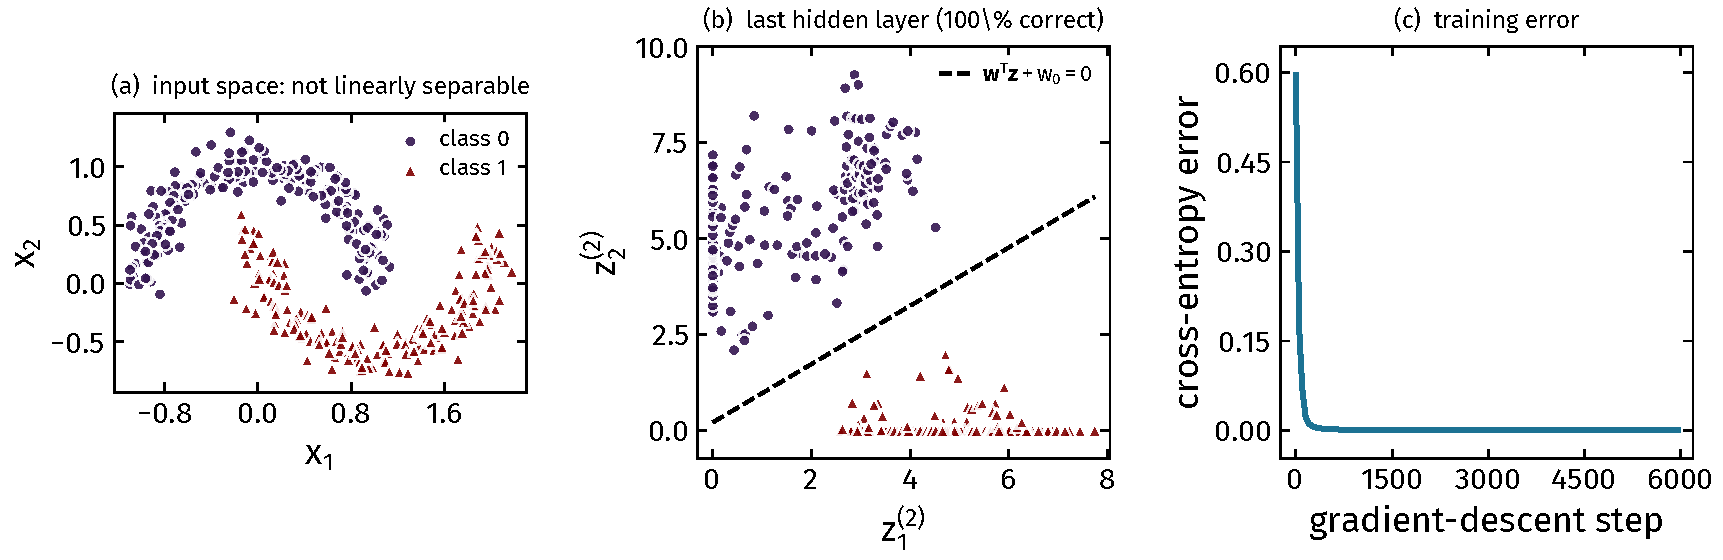
\includegraphics[height=0.48\textheight]{representation}
  \end{center}
  \figcap[0.96]{(a) the data in input space --- no straight line
  separates the classes. (b) the same points in the coordinates
  $(z^{(2)}_1,z^{(2)}_2)$ of the last hidden layer; dashed is the
  output layer's boundary. (c) the error over training.}
  \vspace{0.1em}
  {\footnotesize
  \begin{itemize}\setlength{\itemsep}{0pt}
    \item The network has \alert{rearranged the data} until a line
          is enough \hfill{\scriptsize cf.\ B\&B, \S6.3.3}
  \end{itemize}}
\end{frame}

\begin{frame}{What that experiment shows}
  \vspace{0.2em}
  \begin{itemize}\setlength{\itemsep}{5pt}
    \item Each layer \alert{transforms} the data to make the task
          easier for the next one
    \item By the final hidden layer the classes are arranged so a
          \alert{linear} classifier suffices --- which is all the
          output layer ever was
    \item That layer's output is the \alert{learned representation}
          (the \emph{embedding}) \hfill{\scriptsize B\&B, \S6.3.3}
    \item Nobody designed those coordinates --- they were
          \alert{learned from the data}
  \end{itemize}
  \shpar{one transform, then a linear read-out}
        {\emph{many} learned transforms, then a linear read-out}
\end{frame}

\begin{frame}{Why depth tends to win in practice}
  \vspace{0.2em}
  \begin{itemize}\setlength{\itemsep}{5pt}
    \item Real data is \alert{compositional}: edges $\to$ shapes
          $\to$ objects; phonemes $\to$ words $\to$ meaning
    \item Deep networks mirror this --- each layer builds
          \alert{features of the previous layer's features}
    \item Fewer parameters for the same function means
          \alert{better generalisation} and less data needed
    \item Caveat: depth alone is not enough --- training deep
          networks needs the tools of the coming classes
          (initialisation, normalisation, residual connections)
  \end{itemize}
  \shpar{flat: features of the raw input}
        {hierarchical: features of features of features}
\end{frame}

\begin{frame}{Takeaways}
  \vspace{0.1em}
  {\footnotesize
  \begin{enumerate}\setlength{\itemsep}{2pt}
    \item A \alert{deep network} is shallow networks
          \alert{composed}: each layer is a linear map followed by
          an activation
    \item Composition \alert{folds} the input, so pieces
          \alert{multiply} rather than add --- at most $pq$ from
          $p$ and $q$, which is why $6$ units gave $12$ pieces
    \item \alert{Universal approximation} holds in $D$ dimensions
          for any non-polynomial activation, by reducing to the
          one-dimensional case through \alert{ridge functions}
    \item Universality does not favour depth: ReLU networks compute
          exactly the continuous piecewise-linear functions,
          shallow or deep. \alert{Efficiency} does --- the sawtooth
          needs $O(L)$ units deep and $2^{L}-1$ shallow
    \item Depth suits \alert{compositional} data by building
          hierarchical, distributed representations
  \end{enumerate}}
  \vspace{-0.1em}
  \begin{redhighlight}
    {\scriptsize Next: how to actually \alert{train} these networks
    --- backpropagation and gradient-based optimisation.}
  \end{redhighlight}
\end{frame}

\begin{frame}{References}
  \footnotesize
  \begin{itemize}\setlength{\itemsep}{2pt}
    \item C.~M.~Bishop \& H.~Bishop. \textit{Deep Learning:
          Foundations and Concepts.} Springer, 2024. Ch.~6 ---
          recursive construction, layer counting, hierarchical and
          distributed representations, representation learning.
          Figure~6.8 reproduced with attribution.
    \item S.~J.~D.~Prince. \textit{Understanding Deep Learning.}
          MIT Press, 2023. Ch.~4 --- composition, folding, region
          counting.
    \item G.~Cybenko, \textit{Math.\ Control Signals Systems} 2:303,
          1989; K.~Hornik, \textit{Neural Networks} 4:251, 1991 ---
          universal approximation.
    \item M.~Leshno, V.~Lin, A.~Pinkus \& S.~Schocken,
          \textit{Neural Networks} 6:861, 1993 --- non-polynomial
          activations.
    \item M.~Telgarsky, \textit{COLT}, 2016 --- depth--width
          separation; G.~Mont\'ufar et al., \textit{NeurIPS}, 2014
          --- linear-region bounds; R.~Arora et al., \textit{ICLR},
          2018 --- ReLU networks and piecewise-linear functions.
    \item All plots generated by \texttt{src/build\_all.py};
          one module per figure under \texttt{src/figures/}.
  \end{itemize}
\end{frame}

\begin{frame}[standout]
  Questions?
\end{frame}

\end{document}
